\chapter{Performance and analysis}
\renewcommand{\baselinestretch}{\mystretch}
\label{chap:Perf}
%\setlength{\parindent}{0pt}

\PARstart{\ca{I}}{\ca{n}} \ca{this chapter, the performances of different implementations were compared. Video encoding formats were also analysed, in order to find an optimal encoding format for exported sequences.}

\section{Playback engine}

\fref{fig:playback} shows the performance of the \ca{new} playback engine \ca{on the same Microsoft Windows-based platform} using \ca{an exported} ``Raw'' sequence. At the first and the last few seconds, the playback engine stopped, the original execution engine was used instead during idle state. The execution engine still uses around $30 \%$ of CPU time during idle; but as soon as playback started, CPU usages drops to around $6 \%$ with stable refresh frame rates. \ca{The new playback engine requires much less computational power compared to the original execution engine.}

\begin{figure}[t]
  \centering
  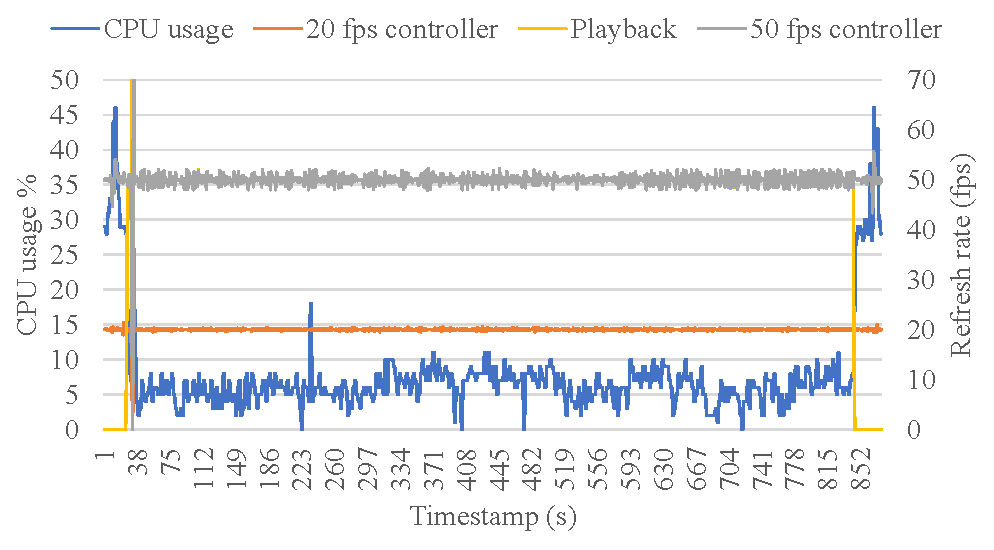
\includegraphics[width=0.8\columnwidth]{Figs/playback.eps}
  \caption{\footnotesize Performance of the new playback engine on Microsoft Windows}
  \label{fig:playback}
\end{figure}

\section{Console application}

\ca{For Linux-based platforms, the console application \texttt{VixenConsole} was used for various performance analysis.}

\subsection{Loading performance}

On an embedded platform with limited \ca{computational} power, the loading time of \texttt{VixenConsole} and all controller modules can take a significant time. The implemented \texttt{tidy} operation can reduce a small portion of the loading time, by remove unused settings for elements and filters\ca{, which} also reduces the size of XML \ca{configuration files}.

However, it still takes \ca{about 30 seconds} from starting \texttt{VixenConsole} to \ca{be able to render} on the \ca{Raspberry Pi B} platform\ca{, in contract to only 5 seconds on the Raspberry Pi 3B platform}. This loading time is for the mono runtime to preform some necessary tasks such as dynamic \ca{recompilation}, \ca{and is} unavoidable.

\subsection{Execution performance}

\fref{fig:raw-seq-p-c} compares the performance between \texttt{VixenLinky} and \texttt{VixenConsole} on multiple platforms. The performance comparison was done by \ca{unlimiting} the playback and controller refresh rate separately using both \texttt{VixenLinky} and \texttt{VixenConsole} applications\ca{;} a total of \ca{four} tests on each of the platforms. The refresh rate data over the entire sequence time \ca{is} then summarised \ca{using} a five-number summary representation, i.e. sample minimum, lower quartile, median, upper quartile and sample maximum. The mean values were also plotted as points. The refresh rate axis is log scale, to focus on the lower performance figures over all platforms.

\begin{figure}[t]
  \centering
  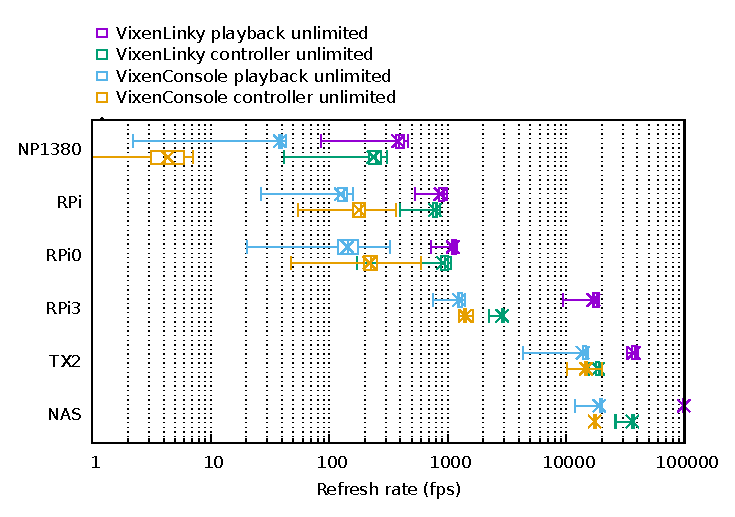
\includegraphics[width=0.9\textwidth]{Figs/raw-seq-p-c.eps}
  \caption{\footnotesize Performance comparison between \texttt{VixenLinky} and \texttt{VixenConsole}}
  \label{fig:raw-seq-p-c}
\end{figure}

By separating playback and controller update tests, the two major performance limitation factors of file IO and processing power can be separately tested.

The figure shows \ca{that} \texttt{VixenConsole} runs a few times slower than the minimal implementation \texttt{VixenLinky}. On NP1380, the controller refresh rate drops below 10 fps, unusable for a 50 fps sequence. It still performs adequately on Raspberry Pi B\ca{;} both the maximum possible playback and controller refresh rate were significantly higher than 50 fps.

\ca{\section{Analysis}}

The mono profiler was used in an attempt to \ca{further optimise the \texttt{VixenConsole} application} on \ca{the} Raspberry Pi B platform. However, it was not particularly \ca{successful}. As shown \ca{in} \lref{lst:mono_sample}, \ca{there are not any significant performance optimisation opportunities available. The} thread sleeping method, \ca{IO read} methods and update methods are all \ca{mandatory and} just as expected. Some overheads from copying command arrays do show up on the summary as array coping methods, but they are \ca{insignificant, also} unavoidable for controller module interface compatibility.

\begin{lstlisting}[float,floatplacement=ht,language=,label=lst:mono_sample,captionpos=b,caption={\footnotesize Summary of time spent in each method, collected by mono profiler}]
Method call summary
Self(ms)   Calls Method name
 584540   38673 System.Threading.Thread:SleepInternal (int)
 520043    2604 System.IO.InotifyWatcher:ReadFromFD (intptr,byte[],intptr)
 410638   21047 System.Threading.WaitHandle:WaitOne_internal (intptr,int)
  63712   19119 Vixen.Sys.Playback:ReadFrame ()
  56368   21044 VixenModules.Output.TCPLinky.TCPLinky:UpdateState (int,Vixen.Commands.ICommand[])
  18617   41132 System.IO.MonoIO:Read (intptr,byte[],int,int,System.IO.MonoIOError&)
  16052  114460 object:__icall_wrapper_ves_icall_array_new_specific (intptr,int)
  12287   49221 System.Array:FastCopy (System.Array,int,System.Array,int,int)
  11344   21044 System.Net.Sockets.Socket:Send_internal (intptr,byte[],int,int,System.Net.Sockets.SocketFlags,int&,bool)
   7274    3020 System.Runtime.CompilerServices.RuntimeHelpers:SufficientExecutionStack ()
\end{lstlisting}

\section{Platform comparison}

\fref{fig:raw-seq-p-c} clearly shows the relative performance figures of all testing platforms. The NP1380 platform is unable to meet the minimum requirement of 50 fps sequences\ca{. Therefore, it was excluded from \texttt{VixenConsole} performance and video format analysis.}

\section{Video formats}

\subsection{Benefits and limitations}

The first noticeable benefit \ca{of encoding an exported sequence to a video file} was reduction in sequence file size. The ``Raw'' sequence format was implemented without any compression algorithm, \ca{and} always has a size linear to total sequence time and channel count. The video formats reduced the sequence size to around $\nicefrac{1}{10}$ of the ``Raw'' sequence. \tref{tbl:size} compares file sizes in different formats of the same example sequence.

\begin{table}[t]
  \centering
  \begin{tabular}{l|l|l}
    \hline
    \textbf{Type} & \textbf{Sequence size} & \textbf{With audio} \\ \hline
    \hline
    Editable sequence                                 & 8.88 MiB  & 24.4 MiB  \\ \hline
    \hline
    50 fps exported \texttt{Raw} sequence             & 337 MiB   & 352 MiB   \\ \hline
    50 fps \texttt{rgb24} encoded video (lossless)    & 26.6 MiB  & 42.5 MiB  \\ \hline
    50 fps \texttt{yuv444p} encoded video (lossless)  & 26.6 MiB  & 42.5 MiB  \\ \hline
    50 fps \texttt{yuv420p} encoded video (lossy)     & 18.2 MiB  & 34.1 MiB  \\ \hline
  \end{tabular}
  \caption{\footnotesize File size comparison of different formats}
  \label{tbl:size}
\end{table}

Using the video format, the exported sequence, audio and configuration information are combined into a single file. This reduction of file count can sometimes simplify the management and sharing of multiple sequences. However, an unexpected limitation on metadata length was encountered on Raspberry Pis. The \texttt{libav} fork of \texttt{ffmpeg} provided by the raspbian distribution of version \texttt{jessie} has an arbitrary limitation of 1000 characters for metadata field length, not enough for all XML configuration information. To work around this issue, some inactive fields of the XML configuration was removed for Raspberry Pis. To completely remove this issue, newer version of \texttt{ffmpeg} without this limitation can be compiled for Raspberry Pis.

The \texttt{yuv420p} encoded video listed in \tref{tbl:size} were transcoded from the \texttt{rgb24} encoded video using the \texttt{ffmpeg} command-line tool. This \ca{shows} another benefit of using a video file. All tools developed for general purpose video processing, editing and filtering can also be used for the exported sequences.

With these sophisticated video \ca{compression} algorithms, a drop of the sequence loading speed was expected. Fortunately, the \texttt{ffmpeg} library is capable of utilising media acceleration features to speed up video decoding, such as SIMD instructions and dedicated video decoding hardware. However, a \ca{low} resolution video, such as the $76 \times 76$ video from \fref{fig:video-info}, is more than capable of supporting thousands of controller channels. It may not leverage the full advantage of dedicated high resolution hardware video decoding accelerators.

\subsection{Encoding formats}

\begin{figure*}[t]
  \centering
  \subfloat[Packed \texttt{RGB}]{\includegraphics[width=0.3\textwidth]{Figs/video/rgb24-raw-scale.png}%
  \label{fig:video-rgb}}\hfil
  \subfloat[Packed \texttt{YUV}]{\includegraphics[width=0.3\textwidth]{Figs/video/yuv-scale.png}%
  \label{fig:video-yuv}}\hfil
  \subfloat[Planar \texttt{YUV}]{\includegraphics[width=0.3\textwidth]{Figs/video/y-u-v-scale.png}%
  \label{fig:video-yuvp}}\\
  %\subfloat[Constant rate factor 6]{\includegraphics[width=0.3\textwidth]{Figs/video/rgb24-6-scale.png}}\hfil
  %\subfloat[Difference blend]{\includegraphics[width=0.3\textwidth]{Figs/video/rgb24-6-scale-diff.png}}\hfil
  %\subfloat[XOR blend]{\includegraphics[width=0.3\textwidth]{Figs/video/rgb24-6-scale-xor.png}}\\
  \subfloat[Constant rate factor 12]{\includegraphics[width=0.3\textwidth]{Figs/video/rgb24-12-scale.png}}\hfil
  \subfloat[Difference blend]{\includegraphics[width=0.3\textwidth]{Figs/video/rgb24-12-scale-diff.png}}\hfil
  \subfloat[XOR blend]{\includegraphics[width=0.3\textwidth]{Figs/video/rgb24-12-scale-xor.png}}\\
  \subfloat[Constant rate factor 24]{\includegraphics[width=0.3\textwidth]{Figs/video/rgb24-24-scale.png}}\hfil
  \subfloat[Difference blend]{\includegraphics[width=0.3\textwidth]{Figs/video/rgb24-24-scale-diff.png}}\hfil
  \subfloat[XOR blend]{\includegraphics[width=0.3\textwidth]{Figs/video/rgb24-24-scale-xor.png}}\\
  %\subfloat[Constant rate factor 24]{\includegraphics[width=0.3\textwidth]{Figs/video/yuv444p-24-scale.png}}\hfil
  %\subfloat[Difference blend]{\includegraphics[width=0.3\textwidth]{Figs/video/yuv444p-24-scale-diff.png}}\hfil
  %\subfloat[XOR blend]{\includegraphics[width=0.3\textwidth]{Figs/video/yuv444p-24-scale-xor.png}}\\
  \subfloat[\texttt{yuv420p} encoding]{\includegraphics[width=0.3\textwidth]{Figs/video/yuv420p-0-scale.png}%
  \label{fig:video-420}}\hfil
  \subfloat[Difference blend]{\includegraphics[width=0.3\textwidth]{Figs/video/yuv420p-0-scale-diff.png}%
  \label{fig:video-420-diff}}\hfil
  \subfloat[XOR blend]{\includegraphics[width=0.3\textwidth]{Figs/video/yuv420p-0-scale-xor.png}%
  \label{fig:video-420-xor}}\\
  \caption{\footnotesize Video encoding formats comparison of frame 13850}
  \label{fig:video-pix_fmt}
\end{figure*}

There are several possible ways to encode sequence channel data into a video pixel format. \fref{fig:video-rgb}, \ref{fig:video-yuv} and \ref{fig:video-yuvp} shows 3 different channel orders tested.

For the \texttt{RGB} format, channel data was copied line-by-line into a video frame buffer with \texttt{rgb24} pixel format. The channel data fills sequentially the red, green and blue channels of continuous pixels, also called packed format.

Similarly, \fref{fig:video-yuv} was encoded as packed \texttt{YUV} for comparison. However, only planar pixel format of \texttt{yuv444p} is available for video frames. The frame buffer stores an entire frame of \texttt{Y} channel first, followed by a frame of \texttt{U} and \texttt{V} channels. For the packed \texttt{YUV} format, this requires complex buffer copying routine, \ca{which} may decrease the performance.

\fref{fig:video-yuvp} shows the appearance of storing channel data as planar \texttt{YUV} format \ca{instead}. Because the example sequence contains lots of \texttt{RGB} elements, pixels with similar colours were all separated by two other pixels in the planar format. This separation resulted in lots of sharp pixel boundaries, which can be badly degraded when transcoding to lower quality video settings.

The second and third rows of \fref{fig:video-pix_fmt} show the quality degradation with lower quality settings using the same \texttt{rgb24} pixel format. The increase of the constant quality factor (CRF) means the video data rate will be more restricted and reduced. The frame difference of CRF 12 is hardly visible, but the \texttt{XOR} blend clearly shows there are binary differences to the reference frame.

Within the 3 formats tested, \texttt{yuv420p} probably is the most common video encoding format currently. It is also more commonly supported by hardware video accelerators. However, \texttt{yuv420p} is not capable to store channel data losslessly with the same image resolution. It is more suitable for storing realistic videos, where sudden colour changes between pixels are uncritical and not common. Colour degrade and cross-talk between channels are unavoidable with the \texttt{yuv420p} encoding format, as shown by the last row of \fref{fig:video-pix_fmt}.

\ca{
\tref{tbl:video_format} compares the difference between these video encoding formats. The differences were calculated according to \eref{eq:diff}. The PSNR (Peak Signal to Noise Ratio) values were calculated using the PSNR filter from \texttt{ffmpeg}, which gives a logarithmic indication of errors between two video streams. The table shows that packed \texttt{RGB} gives the smallest file size. Therefore, \texttt{rgb24} was chosen as the optimal pixel format.

\begin{equation}
  \frac{\sum_n^{N_f} \sum_i^{N_c} \left| A_{n,i} - B_{n,i} \right|}{N_f \times N_c \times 256} \%
  \label{eq:diff}
\end{equation}
Where $N_f$ is the number of frames, $N_c$ is the number of channels, $A$ and $B$ are the data from input $A$ and $B$ respectively. $256$ was chosen because all channels in the test sequence are 8-bit channels.
}

\begin{table}[t]
  \centering
  \begin{tabular}{l|l|l|l|l}
    \hline
    \textbf{Type} & \textbf{File size} & \textbf{Data rate} & \textbf{Difference} & \textbf{Average PSNR} \\ \hline
    \hline
    Packed \texttt{RGB} with rgb24     & 26.6 MiB  & 544 kb/s  & -         & -         \\ \hline
    Packed \texttt{YUV} with yuv444p    & 29.5 MiB  & 604 kb/s  & -         & -         \\ \hline
    Planar \texttt{YUV}     & 38.3 MiB  & 784 kb/s  & -         & -         \\ \hline
    \hline
    \texttt{rgb24} CRF 6    & 26.5 MiB  & 539 kb/s  & 0.090 \%  & 48.60     \\ \hline
    \texttt{rgb24} CRF 12   & 20.6 MiB  & 418 kb/s  & 0.189 \%  & 44.40     \\ \hline
    \texttt{rgb24} CRF 24   & 11.8 MiB  & 238 kb/s  & 0.683 \%  & 35.17     \\ \hline
    \texttt{yuv420p} CRF 0  & 18.2 MiB  & 373 kb/s  & 3.323 \%  & 19.66     \\ \hline
  \end{tabular}
  \caption{\footnotesize Comparison between different video encoding formats}
  \label{tbl:video_format}
\end{table}

\subsection{Performance comparison}

\begin{figure*}[t]
  \centering
  \subfloat[Raspberry Pi B]{\includegraphics[width=0.6\textwidth]{Figs/RPi-perf.eps}%
  \label{fig:perf_RPi}}
  \hfil
  \subfloat[Raspberry Pi 3B]{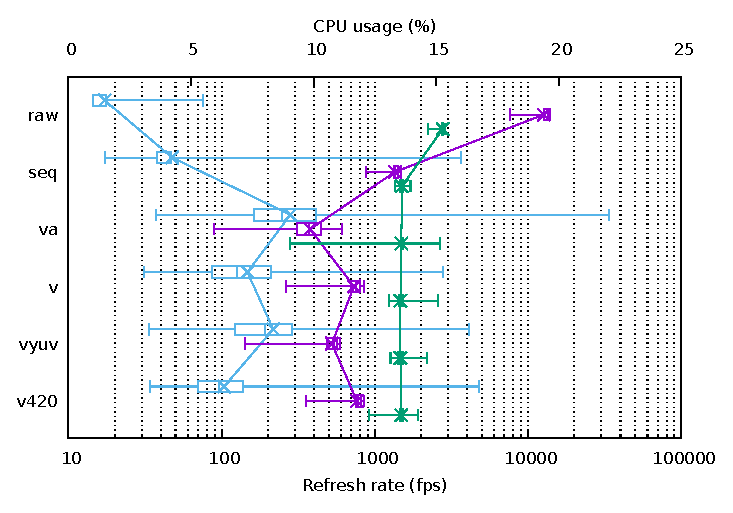
\includegraphics[width=0.6\textwidth]{Figs/RPi3-perf.eps}%
  \label{fig:perf_RPi3}}
  \hfil
  \subfloat[Jetson TX2]{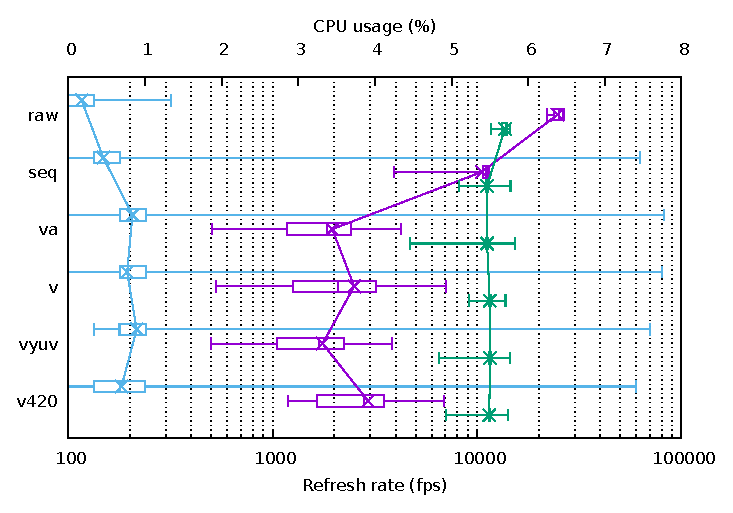
\includegraphics[width=0.6\textwidth]{Figs/TX2-perf.eps}%
  \label{fig:perf_TX2}}
  \caption{\footnotesize Performances of different implementations on different platforms}
  \label{fig:perf}
\end{figure*}

\fref{fig:perf_RPi} shows the performance comparison between different implementations on Raspberry Pi B. \texttt{VixenLinky} (referenced by \texttt{raw}) has the highest refresh rate for its simplicity. \texttt{VixenConsole} with the ``Raw'' sequence format (referenced by \texttt{seq}) has the second highest performance. The unlimited playback performance drops to almost half when using a \texttt{rgb24} encoded video as the input (referenced by \texttt{v}). The performance drops again by a small factor when audio stream was also added to the video input (referenced by \texttt{va}). The video only playback performance of \texttt{yuv420p} encoding (referenced by \texttt{v420}) is only a little bit higher than the lossless \texttt{rgb24} encoding (\texttt{v}), whereas the performance of lossless \texttt{yuv444p} encoding (referenced by \texttt{vyuv}) is noticeably lower. Therefore, video encoding format of \texttt{libx264rgb} with \texttt{rgb24} pixel format is more suitable for encoding video sequences.

\ca{\fref{fig:perf_RPi3} and} \fref{fig:perf_TX2} shows the performance comparison \ca{on two other platforms}, \ca{the Raspberry Pi 3B and} the NVIDIA Jetson TX2 platforms. \ca{The refresh rate easily reached a few hundreds of fps on the Raspberry Pi 3B platform, and more on the TX2 platform, which} has \ca{a} similar single core CPU performance to the Microsoft Windows laptop. \ca{On the TX2 platform, the} maximum refresh rates \ca{reached} over 1,000 fps for playback and 10,000 fps for controllers. For the 50 fps \ca{test} sequence, the CPU usage almost never reaches above $1 \%$. \ca{Compared} to the original Vixen application struggling to \ca{reach a} 50 fps refresh rate on Microsoft Windows, the new playback engine definitely achieved \ca{substantial} performance improvements.

\cmt{Test different container formats?}
